\documentclass[titlepage,a4paper]{article}

\usepackage{a4wide}
\usepackage[colorlinks=true,linkcolor=black,urlcolor=blue,bookmarksopen=true]{hyperref}
\usepackage{bookmark}
\usepackage{fancyhdr}
\usepackage[spanish]{babel}
\usepackage[utf8]{inputenc}
\usepackage[T1]{fontenc}
\usepackage{graphicx}
\usepackage{float}
\usepackage{amsmath}
\usepackage{multirow}
\usepackage{enumitem}
\usepackage{listings}
\usepackage{color}
\usepackage{upgreek}
 
\definecolor{codegreen}{rgb}{0,0.6,0}
\definecolor{codegray}{rgb}{0.5,0.5,0.5}
\definecolor{codepurple}{rgb}{0.58,0,0.82}
\definecolor{backcolour}{rgb}{0.95,0.95,0.92}
 
\lstdefinestyle{mystyle}{
    backgroundcolor=\color{backcolour},   
    commentstyle=\color{codegreen},
    keywordstyle=\color{magenta},
    numberstyle=\tiny\color{codegray},
    stringstyle=\color{codepurple},
    basicstyle=\footnotesize,
    breakatwhitespace=false,         
    breaklines=true,                 
    captionpos=b,                    
    keepspaces=true,                 
    numbers=left,                    
    numbersep=5pt,                  
    showspaces=false,                
    showstringspaces=false,
    showtabs=false,                  
    tabsize=2
}
 
\lstset{style=mystyle}
\lstset{language=Octave}

\pagestyle{fancy}
\fancyhf{}
\fancyhead[L]{TP2 - Grupo 5}
\fancyhead[R]{Análisis Numérico I - FIUBA}
\renewcommand{\headrulewidth}{0.4pt}
\fancyfoot[C]{\thepage}
\renewcommand{\footrulewidth}{0.4pt}


\begin{document}


\begin{titlepage}
	\hfill
\includegraphics[width=6cm]{logofiuba.jpg}
    	\centering
    	\vfill
	\huge \textbf{Análisis Numérico I\\}
	\huge \textbf{[75.12/95.04]\\}
	\huge \textbf{Curso 3\\}
	\huge \textbf{Trabajo Práctico 2}\\
	\huge \textbf{Problema de los Tres Cuerpos Restringido}
	\vskip2cm
	\large
	Grupo 5 \\
    	Primer cuatrimestre de 2019 
	\vfill

	\begin{tabular}{ |l|l|l| }
		\hline
		\multicolumn{3} { |c| } {\textbf{Integrantes del grupo}} \\ \hline
		Santa María Tomás & 92797 & tomasisantamaria@gmail.com\\ \hline
	 	Hemmingsen Lucas & 76187 & lhemmingsen@fi.uba.ar\\ \hline
	 	Huenul Matías & 102135 & matias.huenul.07@gmail.com\\ \hline
	\end{tabular}
	\vfill
    	\vfill
\end{titlepage}

\tableofcontents %Esta línea genera un indice a partir de las secciones y subsecciones creadas en el documento
	\newpage

	
\section{Introducción}\label{sec:introd}
	El objetivo del presente trabajo práctico es utilizar los distintos metodos numéricos de problema de valor inicial 
	para ecuaciones diferenciales ordinarias, para resolver el ``Problema de los Tres Cuerpos Restringido o de Euler'' 
	y realizar una comparación de los resultados con cada método.

	Los métodos que utilizaremos son el método de Euler, Runge-Kutta de orden 2 y 4, Nystr\"om y Newmark.

	


\section{Conceptos teóricos}\label{sec:conceptos}
	\subsection{Método de Euler}
	\subsection{Método de Runge-Kutta}
	\subsection{Método de Nystr\"om}
	\subsection{Método de Newmark}
	\subsection{Sistema de ecuaciones diferenciales}
	\subsection{Ecuaciones diferenciales de orden mayor o igual a 2}

\section{Desarrollo}\label{sec:desarrollo}
	\subsection{Parte A}\label{sec:parteA}

		Tenemos el siguiente sistema de ecuaciones diferenciales de segundo orden que representan el movimiento de un satélite
		viajando entre la tierra y la luna e influenciado gravitatoriamente solo por estos dos cuerpos:
		\begin{equation}
			\begin{cases}
				x''_{1} = 2x'_{2} + x_{1} - \eta\frac{x_{1} + \mu}{d_{1}^{3}} - \mu\frac{x_{1}-\eta}{d_{2}^{3}}\\
				x''_{2} = -2x'_{1} + x_{2} - \eta\frac{x_{2}}{d_{1}^{3}} - \mu\frac{x_{2}}{d_{2}^{3}}
			\end{cases}
		\end{equation}

		Siendo $d_{1}=\sqrt{(x_{1}+\mu)^{2} + x_{2}^{2}}$ y $d_{2}=\sqrt{(x_{1}-\eta)^{2} + x_{2}^{2}}$.

		Sea:

		\begin{equation}
			\begin{cases}
				v_{1}(t) = x'_{1}(t)\\
				v_{2}(t) = x'_{2}(t)
			\end{cases}
		\end{equation}

		Entonces podemos transformar el sistema de ecuaciones anterior en un sistema de cuatro ecuaciones 
		diferenciales de primer orden:

		\begin{equation}
			\begin{cases}
				x'_{1}(t) = v_{1}(t)\\
				v'_{1}(t) = 2v_{2}(t) + x_{1}(t) - \eta\frac{x_{1}(t) + \mu}{d_{1}(t)^{3}} - \mu\frac{x_{1}(t) - \eta}{d_{2}(t)^{3}}\\
				x'_{2}(t) = v_{2}(t)\\				
				v'_{2}(t) = -2v_{1}(t) + x_{2}(t) - \eta\frac{x_{2}(t)}{d_{1}(t)^{3}} - \mu\frac{x_{2}(t)}{d_{2}(t)^{3}}
			\end{cases}
		\end{equation}

		Con valores iniciales en $t=t_{0}$:

		\begin{equation}
			\begin{cases}
				x_{1}(t_{0}) = x_{1_{0}}\\
				v_{1}(t_{0}) = v_{1_{0}}\\
				x_{2}(t_{0}) = x_{2_{0}}\\				
				v_{2}(t_{0}) = v_{2_{0}}\\
			\end{cases}
		\end{equation}

	\subsection{Parte B}\label{sec:parteB}
		Ahora resolvamos el problema numéricamente con la función \emph{lsode} de \emph{Octave}.		
		Primero creamos la función \emph{yprima}, que representa a la función \emph{f(t,y)}.
		A continuación se detalla el código de la misma:

		\lstinputlisting[language=Octave]{yprima.m}

		Luego, desde la consola de \emph{Octave} ejecutamos la función \emph{lsode} con la función 
		\emph{yprima} como entrada, con una posición inicial $(x_{1}, x_{2}) = (1.2, 0)$ y velocidad inicial 
		$(v_{1}, v_{2}) = (0, -0.8)$ en el intervalo $[t_{0}, t_{1}) = [0, 2]$ con un $h=0.01$.
		Para ello, ejecutamos:

			\begin{lstlisting}
				[y]=lsode('yprima',[1.2 0 0 -0.8],0:0.01:2)			
			\end{lstlisting}
		con lo que en la última iteración (en t=2) obtenemos una posición final 
		$(x_{1}, x_{2}) = (-0.51306, 0.07881)$ y una velocidad final $(v_{1}, v_{2}) = (-1.18383, -0.48564)$.

		A continuación se muestra un gráfico de la trayectoria del satélite, que se mueve desde el extremo
		derecho del gráfico hacia la izquierda.
		
		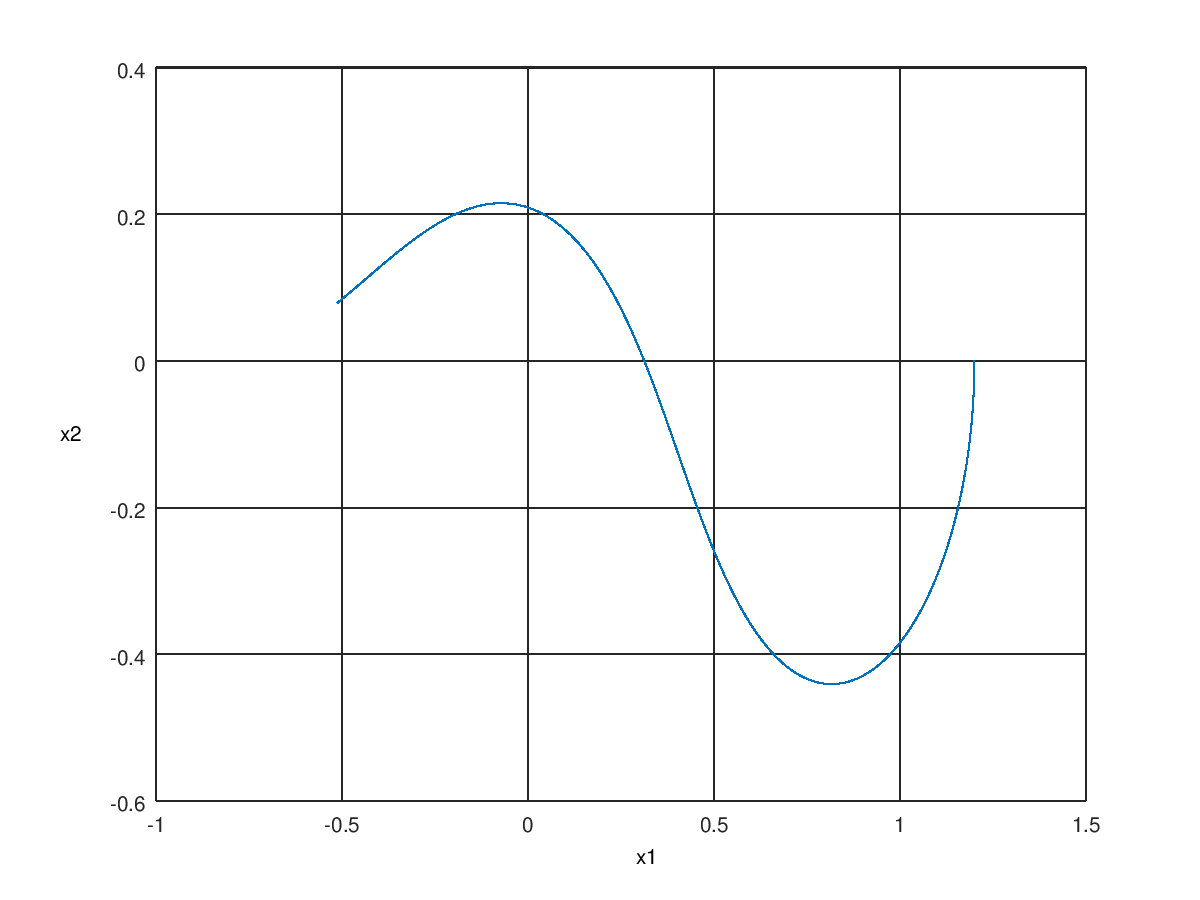
\includegraphics[width=\textwidth]{parteb.png}

	\subsection{Parte C}\label{sec:parteC}
		

	\subsection{Parte D}\label{sec:parteD}

	\subsection{Parte E}\label{sec:parteE}

	\subsection{Parte F}\label{sec:parteF}

	\subsection{Parte G}\label{sec:parteG}

\section{Conclusiones}\label{sec:conc}


\begin{thebibliography}{9} 
	
	 
\end{thebibliography}



\end{document}